        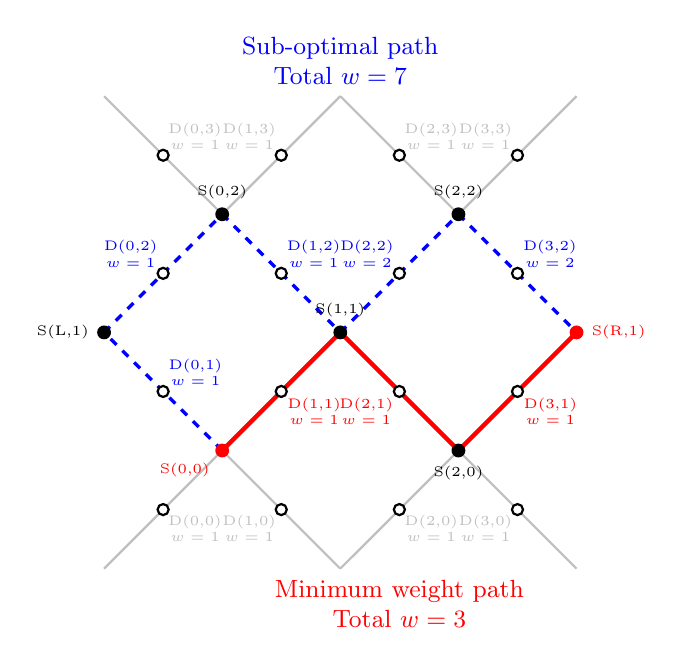
\begin{tikzpicture}[scale=1.5]
            % Styles matching the new sizing and background removal
            \tikzset{
                syndrome/.style={circle, fill=black, inner sep=0pt, minimum size=5pt},
                defect/.style={circle, fill=red, inner sep=0pt, minimum size=5pt},
                edge/.style={gray!50, thick},
                edge_marker/.style={circle, draw=black, fill=white, thick, inner sep=0pt, minimum size=4pt},
                lbl/.style={font=\tiny, align=center, inner sep=1.5pt}
            }
            
            % Perfect 45-degree mathematical coordinates
            \coordinate (C00) at (0.5, 0.5);
            \coordinate (C20) at (2.5, 0.5);
            \coordinate (C11) at (1.5, 1.5);
            \coordinate (C02) at (0.5, 2.5);
            \coordinate (C22) at (2.5, 2.5);
            \coordinate (CHL) at (-0.5, 1.5); % Aligned to logical grid
            \coordinate (CHR) at (3.5, 1.5);  % Aligned to logical grid

            % 8 Boundary edges terminating at the virtual boundaries
            \foreach \start/\dest/\dlabel/\pos in {
                C00/{-0.5, -0.5}/{D(0,0)}/below right,
                C00/{1.5, -0.5}/{D(1,0)}/below left,
                C20/{1.5, -0.5}/{D(2,0)}/below right,
                C20/{3.5, -0.5}/{D(3,0)}/below left,
                C02/{-0.5, 3.5}/{D(0,3)}/above right,
                C02/{1.5, 3.5}/{D(1,3)}/above left,
                C22/{1.5, 3.5}/{D(2,3)}/above right,
                C22/{3.5, 3.5}/{D(3,3)}/above left%
            } {
                \draw[edge] (\start) -- (\dest) node[midway, edge_marker] {} node[midway, \pos, lbl] {\dlabel\\$w=1$};
            }

            % Path 2 (Sub-optimal, blue dashed)
            \foreach \start/\dest/\dlabel/\weight/\pos in {
                C00/CHL/{D(0,1)}/1/above right,
                CHL/C02/{D(0,2)}/1/above left,
                C02/C11/{D(1,2)}/1/above right,
                C11/C22/{D(2,2)}/2/above left,
                C22/CHR/{D(3,2)}/2/above right%
            } {
                \draw[blue, dashed, very thick] (\start) -- (\dest) node[midway, solid, edge_marker] {} node[midway, \pos, lbl, text=blue] {\dlabel\\$w=\weight$};
            }

            % Path 1 (Optimal, red solid)
            \foreach \start/\dest/\dlabel/\weight/\pos in {
                C00/C11/{D(1,1)}/1/below right,
                C11/C20/{D(2,1)}/1/below left,
                C20/CHR/{D(3,1)}/1/below right%
            } {
                \draw[red, ultra thick] (\start) -- (\dest) node[midway, edge_marker] {} node[midway, \pos, lbl, text=red] {\dlabel\\$w=\weight$};
            }

            % Place the 7 graph nodes covering the ends of the lines
            \node[syndrome] at (C20) {}; \node[below=2pt, font=\tiny] at (C20) {S(2,0)};
            \node[syndrome] at (C11) {}; \node[above=2pt, font=\tiny] at (C11) {S(1,1)};
            \node[syndrome] at (C02) {}; \node[above=2pt, font=\tiny] at (C02) {S(0,2)};
            \node[syndrome] at (C22) {}; \node[above=2pt, font=\tiny] at (C22) {S(2,2)};
            \node[syndrome] at (CHL) {}; \node[left=2pt, font=\tiny] at (CHL) {S(L,1)};
            
            % Highlight the active defects in red
            \node[defect] at (C00) {}; \node[below left=1pt, font=\tiny, text=red] at (C00) {S(0,0)};
            \node[defect] at (CHR) {}; \node[right=2pt, font=\tiny, text=red] at (CHR) {S(R,1)};

            % Display total path weights
            \node[blue, font=\small, align=center] at (1.5, 3.8) {Sub-optimal path\\Total $w=7$};
            \node[red, font=\small, align=center] at (2.0, -0.8) {Minimum weight path\\Total $w=3$};
            
        \end{tikzpicture}
